\documentclass[11pt]{article}
\usepackage{matt}
\begin{document}

\section*{Update for the Week of \today}

\begin{figure}[h]
  \centering
  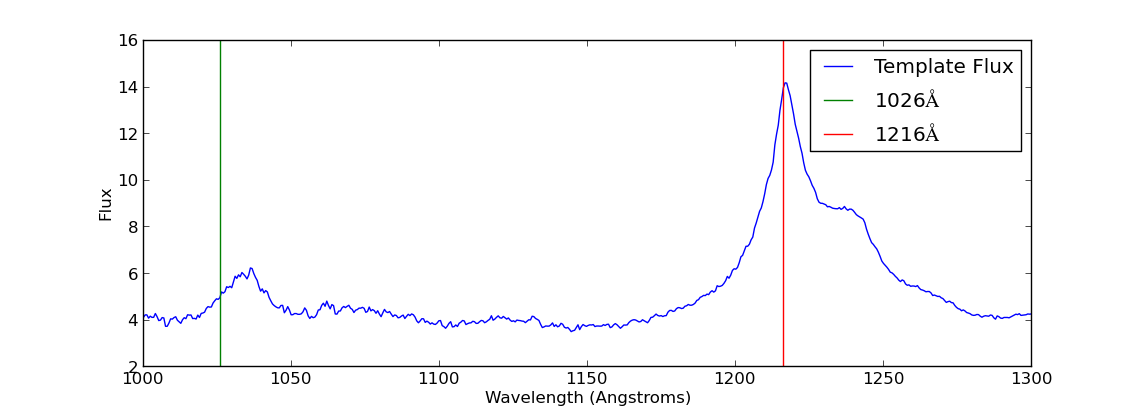
\includegraphics[width=15cm]{QSOTemplateCheck.png}
  \caption{The above figure shows the quasar template from {\tt LBQS.lis}. We also show the \lya\ line and the \lyb\ line. The emission line at $\sim 1070$\AA\ does not appear to match up with the \lyb\ line.}
  \label{fig:todo}
\end{figure}

\begin{figure}[h]
  \centering
  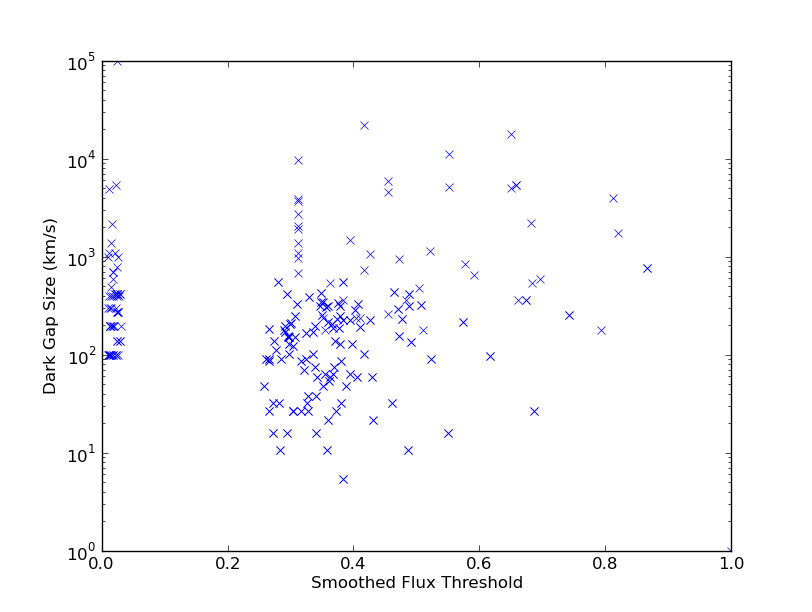
\includegraphics[width=8cm]{LvsT.png}
  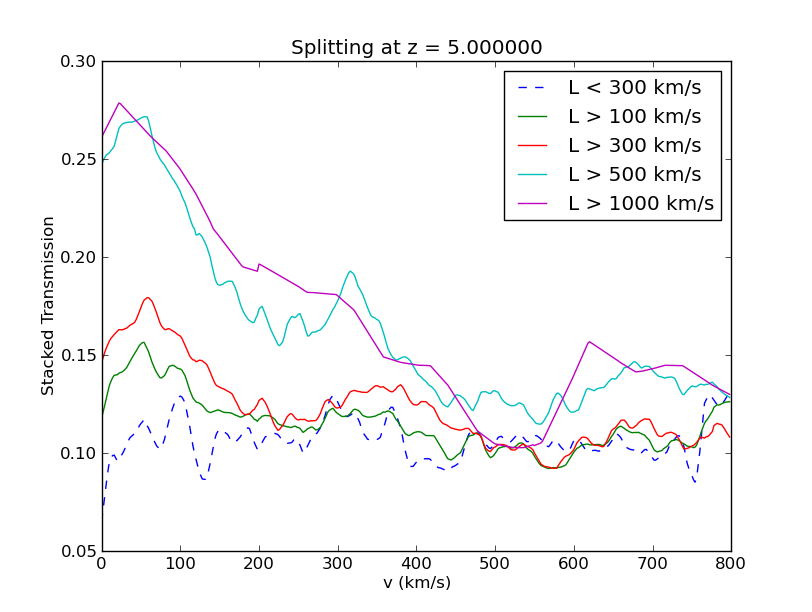
\includegraphics[width=8cm]{Stack_Zgreaterthan5.png}
  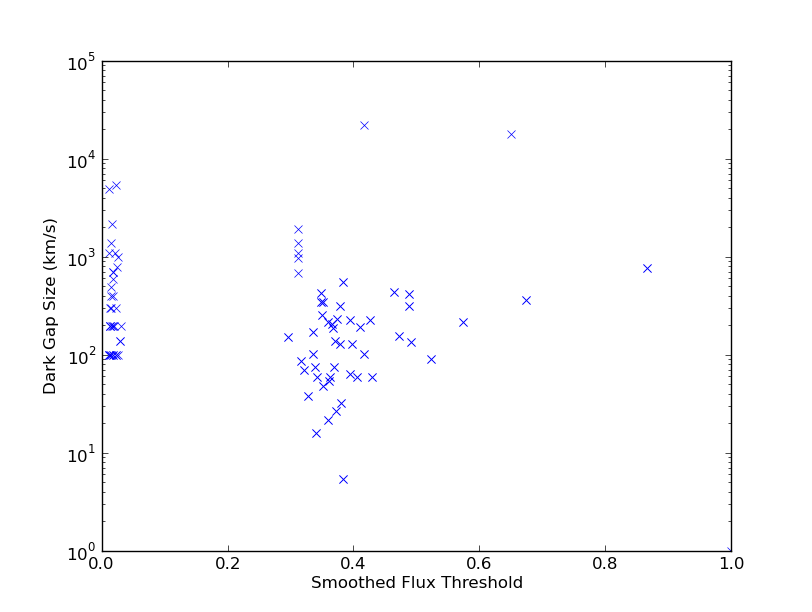
\includegraphics[width=8cm]{LvsT_zGreaterThan5p5.png}
  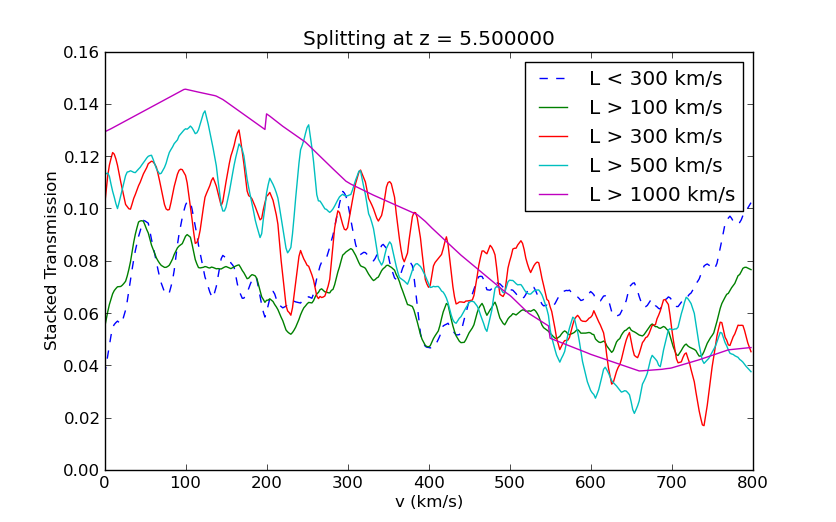
\includegraphics[width=8cm]{Stack_Zgreaterthan5p5.png}
  \caption{Left-hand plots are not correct.}
  \label{fig:todo}
\end{figure}


\begin{figure}[h]
  \centering
  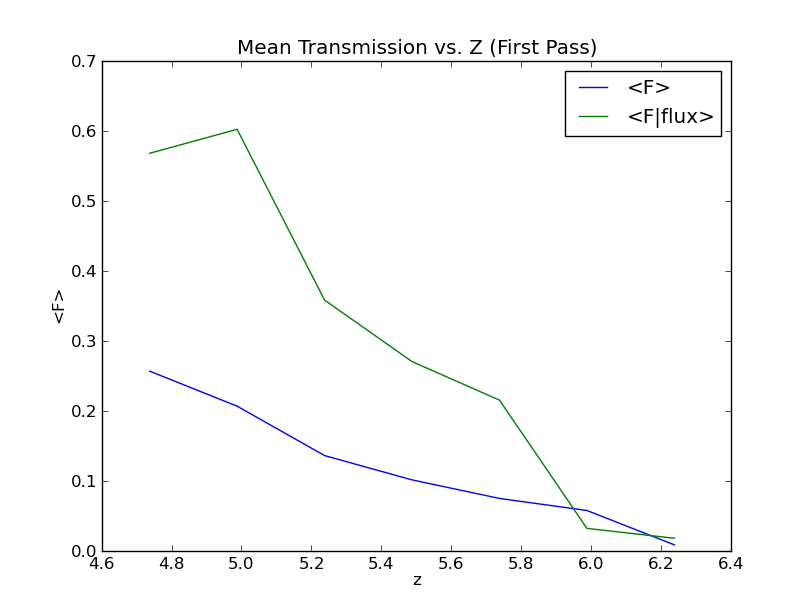
\includegraphics[width=8cm]{meanFs.png}
  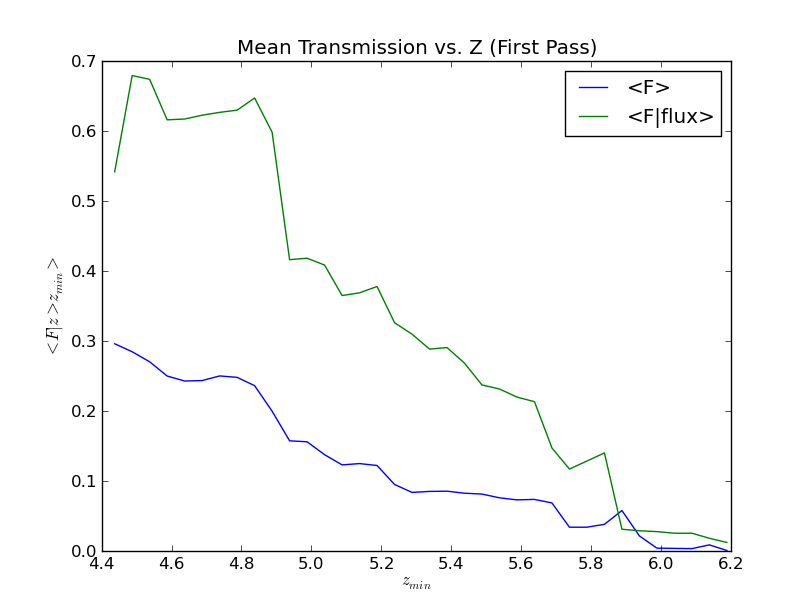
\includegraphics[width=8cm]{FluxCDF.png}
  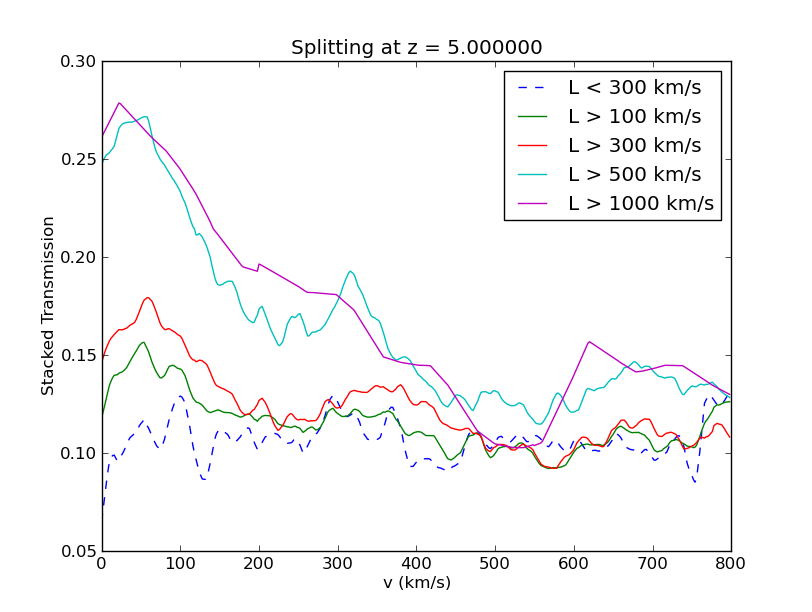
\includegraphics[width=8cm]{Stack_Zgreaterthan5.png}
  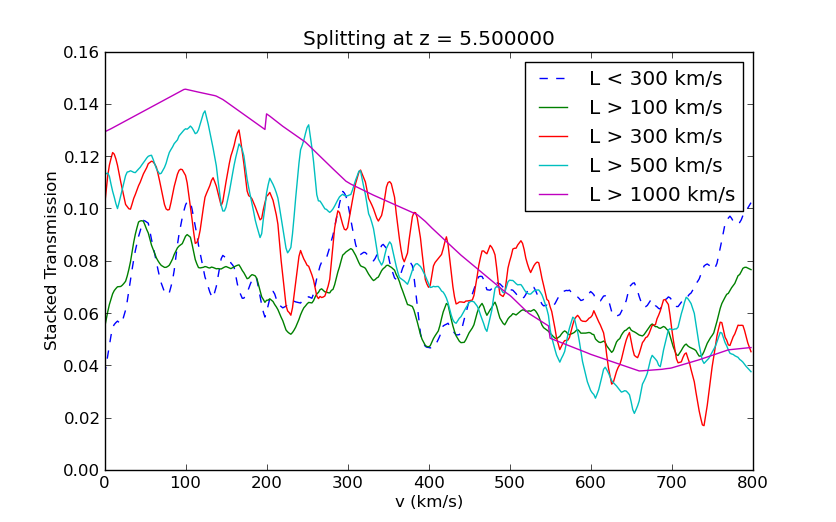
\includegraphics[width=8cm]{Stack_Zgreaterthan5p5.png}
  \caption{todo}
  \label{fig:todo}
\end{figure}


\end{document}